% status: 70
% chapter: TBD

\title{Abstract File System}


\author{Swarnima Sowani}
\affiliation{%
  \institution{Indiana University}
  \streetaddress{Smith Research Center}
  \city{Bloomington} 
  \state{IN} 
  \postcode{47408}
}
\email{shsowani@iu.edu}

\author{Gregor von Laszewski}
\affiliation{%
  \institution{Indiana University}
  \streetaddress{Smith Research Center}
  \city{Bloomington} 
  \state{IN} 
  \postcode{47408}
  \country{USA}}
\email{laszewski@gmail.com}


% The default list of authors is too long for headers}
\renewcommand{\shortauthors}{G. v. Laszewski}


\begin{abstract}
bstract File System is a web services package that implements and abstracts
the underlying storage services and provides a uniform web services APIs for
users to do file operations like, retrieving, storing, removing  etc. The
services are provided to support storage engines such as Amazon Simple Storage
Service, google drive and virtual machine. This web service package can be
used by different big data applications client to perform file operations with
consolidated data view. 


\end{abstract}

\keywords{hid-sp18-420, File system, abstraction, Amazon S3, Google drive, virtual 
machine}


\maketitle

\section{Introduction}


File system operations is an integral part of the operating system and a
quintessential part of most of the applications that deals with storing,
retrieving or reading the files. Now a days it is likely possible to have data
stored at different locations with different storage systems. Managing all this
data together is a difficult task.

There are numerous storage providers who facilitates their customers to store,
read, write, retrieve and other sorts of file operations, however integrating
with each one of them is a tedious tasks since, understanding and implementing
APIs for each service is a time consuming tasks.

That is why abstract file system comes into picture. Abstract file system
provides a layer of abstraction over the underlying file system so that the
users or customers can integrate storage services as file systems like 
Amazon S3~\cite{hid-sp18-420-amazon-S3}, 
Google Drive~\cite{hid-sp18-420-google-drive} and other services 
without even knowing their real implementation.


\section{Technologies used}
\textbf{Python:}

Python 2.7 is the underlying language that was used to implement all the APIs 
provided by Abstract File System.  There are 3 main python files having 
implementation of file operations to be performed with Amazon S3, Google drive 
and Virtual machine storage respectively. 


Different python modules are used to support the implemented functionality.


Some of the important modules are 

\begin{description}
\item \textbf{Boto3}: 

Boto3 is a software development kit (SDK) that provides AWS interface for 
Python applications. Abstract File System is using Boto3 which is the latest 
version of the SDK provided. Boto 3 supports Python versions 2.6.5, 2.7 and 
3.3 ~\cite{hid-sp18-420-boto}. 
It is used to support Amazon S3 interface with Abstract File System.

\item \textbf{ftplib}:

The ftplib module in Python is used to perform different file opearations on 
virtual machine by connecting to FTP server installed on that 
machine~\cite{hid-sp18-420-FTP}.

\item \textbf{yaml}:

This library is used to read the confog.yaml file used in Abstract File System 
to store the configurations required by different storage engines.


\item \item \textbf{google-api-python-client}:

This is a python specific client library provided by google to handle the 
Google drive APIs.



\item \textbf{Swagger}:

Swagger Codegen is used to generate server side stubs based on the 
abstractFileSystem.yaml file with swagger specifications. Swagger was used to 
enable APIs for accessing storage systems provided in this project.

\end{description}




\section{Supported Storage Engines}
Abstract file system is currently supporting three types of storage engines
which are Amazon S3, Google drive and any virtual machine.

\subsection{Amazon S3}

Amazon S3 stands for Simple Storage Service. It is the most popular storage
service provided by Amazon Web Service. It provides a highly scalable,
reliable, and low latency data storage infrastructure at low costs. Amazon S3
can be used to store and retrieve data of any kind and any amount from 
anywhere.


Amazon S3 is known for its durability and stability. Amazon S3 SLAs claims to
provide 99.999999999\% durability for files stored in its durable 
storage~\cite{hid-sp18-420-amazon-S3}.


Amazon S3 is popularly an object storage, where each file is treated as an
object. Amazon S3 claims no cap on the amount of data that can be stored, that
is why companies who needs scale on the go prefer to choose Amazon S3 as their
file or object storage.


Abstract File System encashes on the scalability and simplicity Amazon S3
provides by abstracting the underlying mechanism and providing a way to users
to store their data into the durable S3 storage.

Figure~\ref{fig:architecture}

\begin{figure}[!ht]
        \centering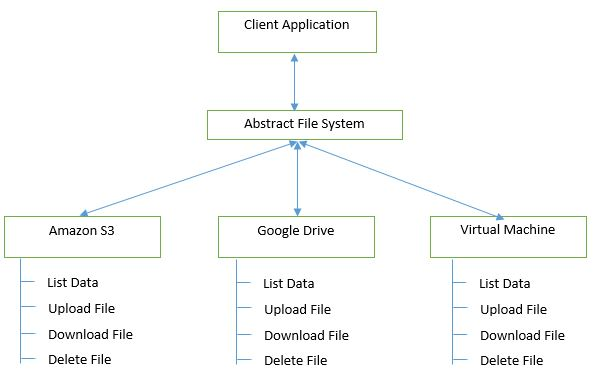
\includegraphics[width=\columnwidth]
        {image/architecture.JPG}
        \caption{System components}\label{fig:architecture}
\end{figure}


As shown in the figure, client applications can interact with abstract file 
system with the web service package provided. With the APis, it will be easy 
to perform file operations such as listing, uploading, downloading and 
deleting in a uniform way with supported storage engines. 

With an abstract layer, all file operations will be like a same process for 
all storage engines and it will be as easy as performing operations on local 
system. 


To get the clear understanding of application, Figure1 figure shows a sample 
wireframe view of simple client application using Abstract File System. 

Figure~\ref{fig:client}

\begin{figure}[!ht]
        \centering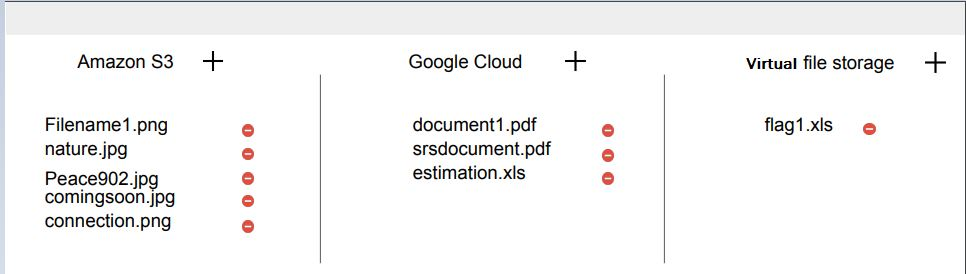
\includegraphics[width=\columnwidth]
        {image/client.JPG}
        \caption{Sample Client Application}\label{fig:client}
\end{figure}



\textbf{File Operations Supported by Abstract File System}


\begin{itemize}
    \item   Listing of files inside a specified bucket (bucket logical
segregation of files)
    \item       Retrieving a specific file
    \item       Storing file in  the specified bucket
    \item       Removing the file from the bucket
\end{itemize}



\textbf{How to enable Amazon S3 as a storage in Abstract File System}


In order to use Amazon S3 as a storage system, first user needs to have an
account with AWS system.


\textbf{Steps to create new root account with AWS}

\begin{enumerate}
    \item Open https://aws.amazon.com/ and click Create New Account.
    \item Give details such as email address, password and user name.
    \item Contact details: Give all specified contact details.
    \item Payment Information: Give credit card or debit card details for user
verification by AWS side.
    \item       Phone verification: AWS will make a call on the given number
and give a 4 digit code to verify your phone number.
    \item Select a support plan and Continue.
\end{enumerate}


\textbf{Steps to create new user in AWS account and giving programmatic access}


\begin{enumerate}
    \item Login to AWS account.
    \item Go to Services and select IAM from drop down. 
	IAM stands for Access and Identity Management.
    \item Inside IAM resources, click on User.
    \item This will show the list of users. Click on Add User to add a new 
user.
    \item Provide user name and select programmatic access.
    \item On next page, provide optional permissions to user such as S3 Full
access and similar.
    \item On next page, review all settings and click Next.
    \item Access key and secret key are displayed here. Save it somewhere safe.
Key file can be downloaded here in \.csv format.
\end{enumerate}



\textbf{To use Amazon S3 as a storage engine within Abstract File System}, AWS
credentials must be provided in the config.yaml file.
Abstract file system requires user to provide 3 parameters to start using S3
service.
\begin{enumerate}
 \item  Access Key
 \item  Secret Key
 \item  AWS region
 \item  Bucket name
\end{enumerate}


Access key and secret key are required for the programmatic authentication for
using S3 services. These keys are provided at the time of account creation of
user.

While creating a new bucket, an AWS region is assigned to that bucket. Though
the buckets are globally unique and can be accessible from anywhere, they are
placed in specific AWS region.
Amazon S3 stores data within resources called bucket. Buckets are logical
segregation of files. Bucket name is configurable from the config.yaml file
which specifies the location where all file operations can be performed.


\subsection{Google Drive}

With 3 billion file uploads every day, Google drive is certainly one of the 
most popular and widely used storage provided by Google. Google drive offers 
its user a storage of 15 gigabytes for free and 100 gigabytes, 1 terabytes, 2 
terabytes, 10 terabytes, 20 terabytes and 30 terabytes through optional paid 
plans. Files uploaded in Google drive can be up to 5 terabytes in size. Google 
drive provides 99.9\% up-time guarantee~\cite{hid-sp18-420-google-drive-wiki}. 

Abstract file system provides integration with Google drive so that they can 
use their existing account or new one to store files seamlessly.

Abstract file system provides integration with Google drive by the means of 
API keys. 

\textbf{File Operations Supported by Abstract File System }
\begin{itemize}
    \item  Listing of files inside a drive
    \item  Retrieving a specific file 
    \item  Storing file inside drive
    \item  Removing the file from drive
\end{itemize}

\textbf{How to enable Google Drive as a storage in Abstract File System}
\\
Abstract file system requires user to login to their google account only for 
the first time of using this application and all later requests will not 
require to authenticate again. 

For the first request to google drive API via Abstract file system, it will 
open a browser for authentication. An existing account or new account with 
google is required for authentication. 

User needs to perform authentication first and then Google drive will ask user 
to allow or deny Abstract File system to access the google drive. 

Figure~\ref{fig:auth}

\begin{figure}[!ht]
        \centering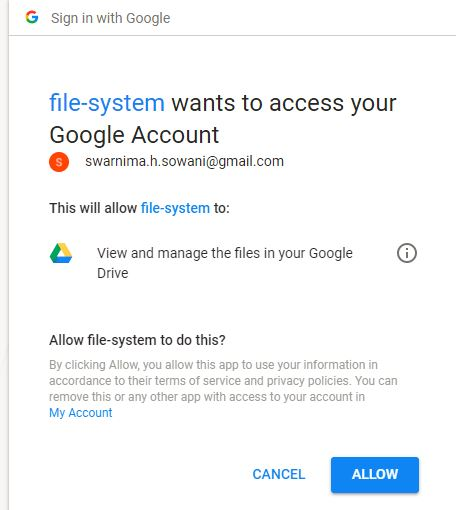
\includegraphics[width=\columnwidth]
        {image/auth.JPG}
        \caption{Aythentication for Google Drive}\label{fig:auth}
\end{figure}


Once user allows access to Abstract File system, user specific API keys will 
be generated and stored inside etc/google-drive-credentials.json file. 
For all later accesses of Abstract file system drive API, these keys will be 
referred and there will be no need to login again. 


\subsection{Virtual Machine}
The virtual machine on any cloud service provider can be used as a storage. In 
certain scenarios, user needs to store the files on their specific servers for 
variety of reasons. Abstract file system facilitates storing the files on the 
server of their choice.

There can be multiple ways to access the storage provided by virtual machines. 

One way is to write an http service accept and transfer file and storage on 
local file system and host this service on the virtual machine. Second way 
could be to do SSH or SCP by writing a sub-process for making a connection to 
machine using machine’s IP, port and authentication through username, 
password or \.pem files. Third way is to do FTP installation on virtual 
machine and using the newly created FTP user in the program to access files on 
the virtual machine.


Abstract File System facilitates integration with any virtual machine by the 
means of ftp installation. FTP is a file transfer protocol and is a standard 
mechanism to deal with remote file operations.


\textbf{File Operations Supported by Abstract File System }
\begin{itemize}
    \item  Listing of files inside a specified folder allowed by ftp
    \item  Retrieving a specific file 
    \item  Storing file inside specified folder
    \item  Removing the file from the folder
\end{itemize}   

\textbf{How to enable Virtual Machine as a storage in Abstract File System}

Here are the steps to install ftp on server~\cite{hid-sp18-420-FTP}
(Ubuntu Linux distribution is taken as example)


\$ sudo apt-get install vsftpd


Edit the configuration file to allow writes to file system as well as set the 
default file system path for file operations as \�/srv/ftp’


\$ sudo service vsftpd restart


Now make the ftp directory ‘/srv/ftp’ writable 


It is required to create a local file system user on the Virtual Machine, you 
can do that by using following command

	
local\_root = /srv/ftp  \\
write\_enable=YES       \\
\$ sudo adduser your\_user\_name    \\


This will ask for password and other details and will create a local user on 
the virtual machine which can access the ftp installations.

Now everything is ready and abstract file system can make connection with the 
file system of virtual machine.


Use config.yaml file in Abstract File System to add the required details of 
Virtual machine. 
It will be required to provide details in config.yaml file– 
\begin{enumerate}
    \item Hostname
    \item Port
    \item Username
    \item Password
\end{enumerate}


Host name is an IP address of the virtual machine which hosts the ftp 
installation. Port number is used to connect to the FTP on given port. By 
default port 21 is used for connection, and finally username and password of 
the FTP user created in FTP installation.





\section{MAIN PROJECT ARTIFACTS}
\subsection{abstractFileSystem.yaml}
This file is used for giving swagger specification for all the APIs used in 
the Abstract File System. This file will be used by Swagger code generator to 
create python stubs as per specification given in the yaml file.
This file contains swagger version, description, base path, path for each APIs 
respective input and output parameters of each API respectively.

\subsection{config.yaml}
This file is used to store the configurations required in the project. 
Config.yaml file is used to store access key, secret key, bucket name and 
region for integrating Amazon S3 in the system. It also stores host name, 
port, username and password required to integrate virtual machine as a storage 
engine in the Abstract File System project.

\subsection{client_id.json}
This file is used by Abstract File system to enable using google drive api in 
the project. This file is generated at the time of registering Abstract File 
System for API of Google drive. It has the key information that enables usage 
of google drive in this application. 

\subsection{google-drive-credentials.json}
This file will store the keys of client who will be using Abstract File 
System. When any drive API is called for first time, it is required to login 
to the google drive and allow Abstract File System to access the user drive. 
After approval, user specific keys will be stored in 
google-drive-credentials.json file

\subsection{MakeFile}
MakeFile has different targets and it is used to build the project. 
Make service is used for performing all the configurations required for 
Abstract File System and then using swagger-codegen to generate code using 
swagger specification file abstractFileSystem.yaml. It will then copy all 
python files to the controller and download the requirements. Make start is 
used to run the service. Make clean is used to clean all the changes done 
while configuring the project. 


MakeFile also supports docker implementation. Make container is used to call 
docker-build and docker-start target which will generate docker container and 
run project services in the new container. Make docker-clean is used to stop 
the service and remove the container. 

\subsection{DockerFile}
DockerFile is used to generate docker image Abstract File System can be run. 
It has specifications required for generating Ubuntu instance along with 
installation of python, java, curl, git, wget and required files to generate 
an image with all required installations ready. It then uses git repository by 
cloning inside image and then running a project based on targets available in 
the make file. 

\subsection{all\_drive\_operations\_controller.py}
This is a python file that contains the code to implement required file 
operations for using Google drive as a storage engine in Abstract File System.

\subsection{all\_s3\_operations\_controller.py}
This is a python file that contains the code to implement required file 
operations for using Amazon S3 as a storage engine in Abstract File System. 

\subsection{all\_vm\_operations\_controller.py}
This is a python file that contains the code to implement required file 
operations for using virtual machine as a storage engine in Abstract File 
System. 


\section{Implementation results}

\textbf{When no configurations done in /etc/config.yaml file, no storage 
system will be accessible.}


Figure~\ref{fig:not-configured}

\begin{figure}[!ht]
        \centering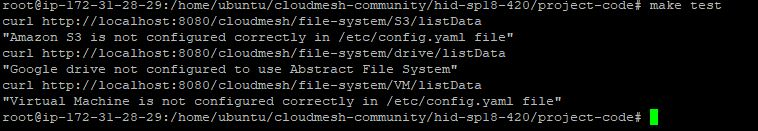
\includegraphics[width=\columnwidth]
        {image/not-configured.JPG}
        \caption{No storage system configured}\label{fig:not-configured}
\end{figure}



\textbf{All files listed from all storage engines }


APIs used:

\begin{itemize}
    \item /cloudmesh/file-system/S3/listData
    \item /cloudmesh/file-system/VM/listData
    \item /cloudmesh/file-system/drive/listData
\end{itemize}

Figure~\ref{fig:make-test}

\begin{figure}[!ht]
        \centering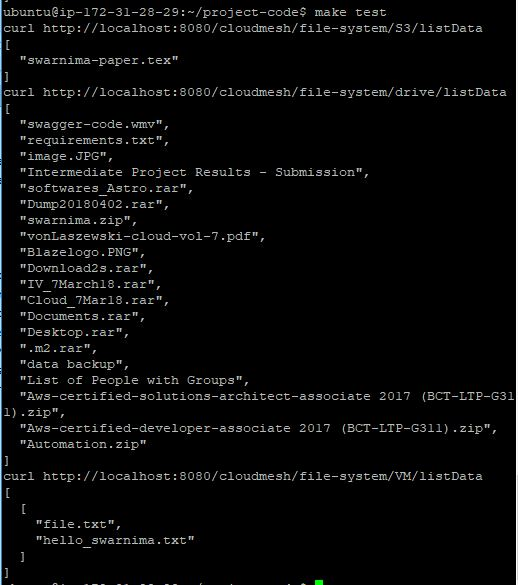
\includegraphics[width=\columnwidth]
        {image/make-test.JPG}
        \caption{all files from all engines}\label{fig:make-test}
\end{figure}


\textbf{All file operations supported by Abstract File System to integrate 
with Amazon S3}

APIs used:

\begin{itemize}
    \item /cloudmesh/file-system/S3/listData
    \item / cloudmesh/file-system/S3/downloadFile/{fileName}
    \item /cloudmesh/file-system/S3/uploadFile/{fileName}
    \item /cloudmesh/file-system/S3/deleteFile/{fileName}
\end{itemize}

Figure~\ref{fig:all-s3}

\begin{figure}[!ht]
        \centering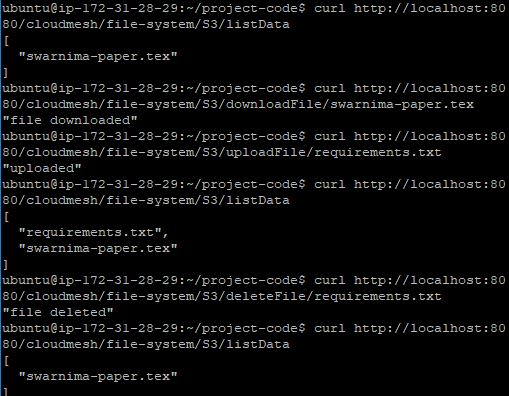
\includegraphics[width=\columnwidth]
        {image/all-s3.JPG}
        \caption{all S3 opearations}\label{fig:all-s3}
\end{figure}


\textbf{All file operations supported by Abstract File System to integrate 
with Virtual Machine storage}


API used:
\begin{itemize}
    \item /cloudmesh/file-system/VM/listData
    \item /cloudmesh/file-system/VM/downloadFile/{fileName}
    \item /cloudmesh/file-system/VM/uploadFile/{fileName}
    \item /cloudmesh/file-system/VM/deleteFile/{fileName}
\end{itemize}

Figure~\ref{fig:VM}

\begin{figure}[!ht]
        \centering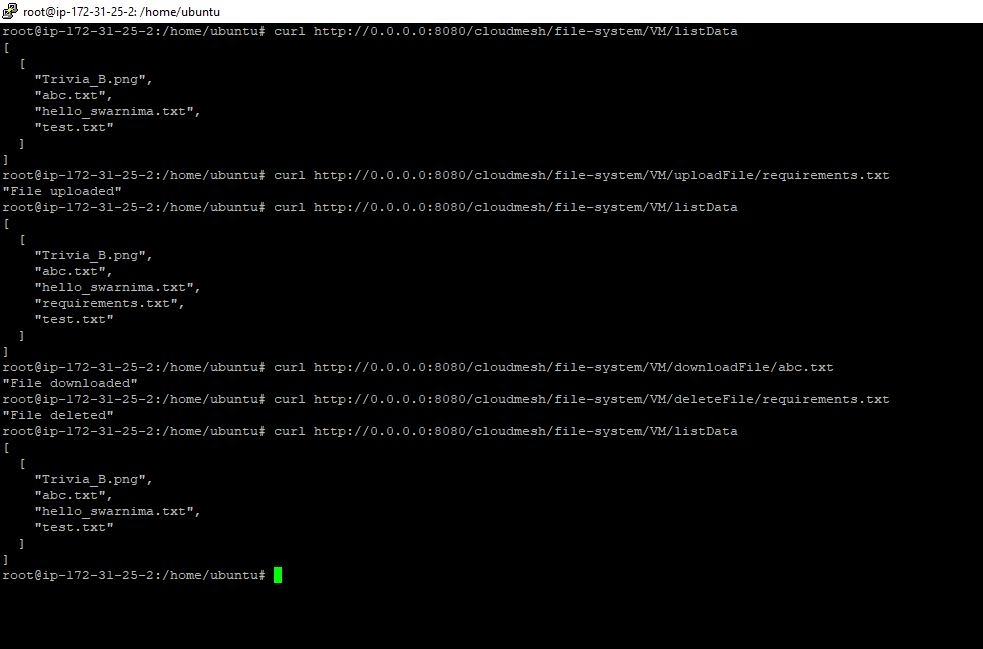
\includegraphics[width=\columnwidth]
        {image/VM.JPG}
        \caption{all VM opearations}\label{fig:VM}
\end{figure}


\textbf{All file operations supported by Abstract File System to integrate 
with Google Drive}


API used:
\begin{itemize}

    \item /cloudmesh/file-system/drive/listData
    \item / cloudmesh/file-system/drive/downloadFile/{fileName}
    \item /cloudmesh/file-system/drive/uploadFile/{fileName}
    \item /cloudmesh/file-system/drive/deleteFile/{fileName}

\end{itemize}

Figure~\ref{fig:drive-upload}

\begin{figure}[!ht]
        \centering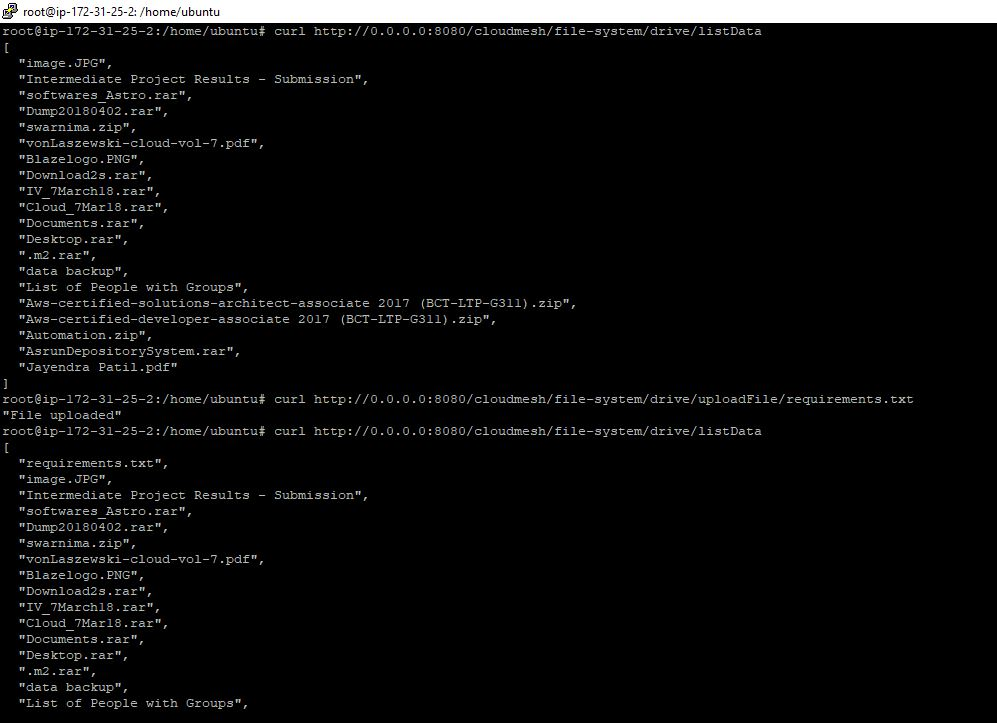
\includegraphics[width=\columnwidth]
        {image/drive-upload.JPG}
        \caption{Drive upload opearations}\label{fig:drive-upload}
\end{figure}


Figure~\ref{fig:drive-delete}

\begin{figure}[!ht]
        \centering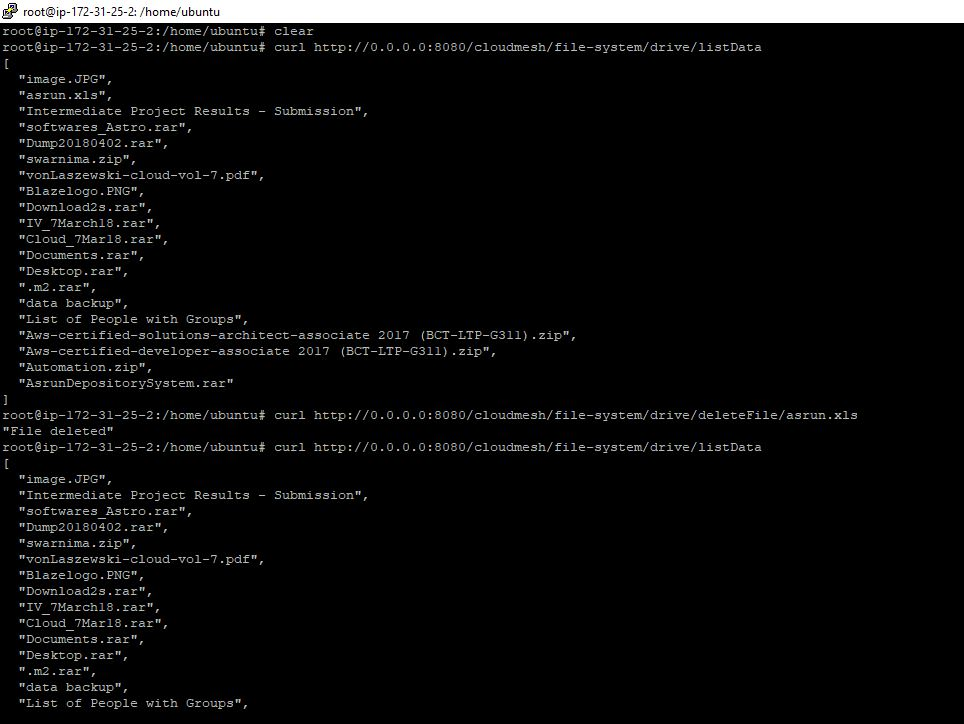
\includegraphics[width=\columnwidth]
        {image/drive-delete.JPG}
        \caption{Drive delete opearations}\label{fig:drive-delete}
\end{figure}


Figure~\ref{fig:drive-download}

\begin{figure}[!ht]
        \centering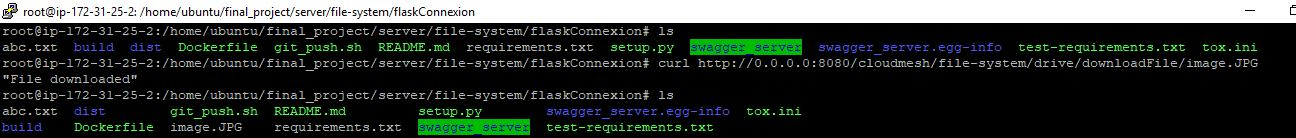
\includegraphics[width=\columnwidth]
        {image/drive-download.JPG}
        \caption{Drive download opearations}\label{fig:drive-download}
\end{figure}


\section{Benefits of Abstract File System}
\begin{enumerate}
    \item Since Abstract File System abstracts the underlying storing 
mechanism, user does not need to know the core implementation of the storage 
services like Amazon S3, Google Drive SDKs etc
    
    \item Switching between underlying storage mechanism is a hassle free task 
and can be done even by a newbie
    
    \item Once the abstract file system is integrated into user’s 
applications, there is no code change required apart from only the 
configuration change to switch the underlying storage mechanism.
    
    \item Scalability is the biggest benefit of the abstract file system, 
since the underlying storage mechanisms can be anything like Amazon S3 which 
provides almost infinite amount of data to be stored and retrieved on demand.
    
\end{enumerate}

\section{Challenges and Scope of improvement}
Abstract File system is currently dealing with only 3 types of storage engines 
which are Amazon S3, Google Drive and Virtual machines. It can be further 
improved to support other storage engines such as Box, DropBox, Azure and many 
more. Abstract File system is scalable and can add other storage systems that 
can be configurable from config.yaml file and writing specific API calls in 
abstractFileSystem.yaml file that will generate stubs to write implementation 
logic. 


Abstract File system is dealing with only file operations right now which are 
listing, uploading, downloading and deleting. It can be improved to add 
directory operations such as create directory, delete directory or sync 
directory operations. 


Current implementation of Abstract File system involved copying files from 
different storage engines to local machine or from local machine to these 
storage systems. An enhancement could include moving files from one storage 
engine to other engine. 



\section{Conclusion}
Abstract File System provides uniform APIs to perform file operations on 
different storage systems in an abstract way. Abstract File System currently 
supports Amazon S3, Google drive and Virtual machine as its storage engine. It 
can be scalable to include other services as well. 


Using Abstract File system, a tedious task to manage files between different 
storage providers will be reduced and client applications can interact with 
different storage engines in a seamless way. 


By using the abstraction layer, storing or retrieving files from different 
storage engines will be same process as being saved locally or transferred 
over the network to other storage system. Such abstraction makes it simpler to 
switch from one system to another without having to rewrite vast swathes of 
application code.




\begin{acks}

  The author would like to thank Dr.~Gregor~von~Laszewski for his
  support and suggestions to write this paper.

\end{acks}

\bibliographystyle{ACM-Reference-Format}
\bibliography{report} 

